
\section{Optimization}
\textbf{Gradient descent update (steepest descent direction)}:
$w^{t+1} = w^t - \eta\nabla_w L(w^t)$
Maximal Stepsize: $\eta \leq \frac{2}{\lambda_{max}}$\quad  $\lambda$: Eigenvalues of $X^TX$ \\
Fastest Stepsize: $\eta = \frac{2}{\lambda_\mathrm{min}+\lambda_\mathrm{max}}$\\
\textbf{Speeding up gradient descent}: 
Momentum (prevent oscillation) $w^{t+1} - w^{t} = \alpha(w^t - w^{t-1}) - \eta\nabla L(w^t)$ \\
Adaptive Methods (AdaGrad, RMSProp, Adam etc.) $w^{t+1}_i = w^t_i - \frac{\eta}{\sqrt{{previouschange}_i + \gamma}}\frac{\partial L}{\partial w_i}(w^t)$ \\
%\textbf{Stochastic Gradient Descent: }
%compute gradients using random subset of points instead of all points\\
\textbf{Convexity}:Guarantees \textcolor{blue}{local = global minimum}\\

1. iff $L(\lambda w + (1-\lambda)v) \leq \lambda L(w) + (1-\lambda)L(v)$;
2. or iff $L(v) \geq L(w) + \nabla L(w)^T(v-w)$ 
3. or iff $\nabla^2L(w)$ positive semi-definite

%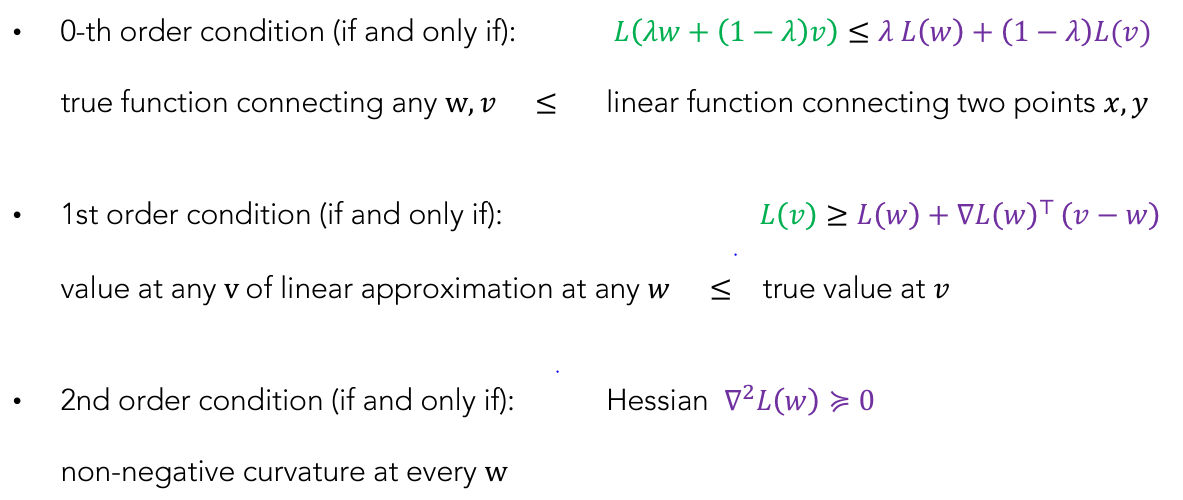
\includegraphics[width=0.8\linewidth]{pics/figure2.PNG}\\
Operation for \textbf{preserving} Convexity:\  if $f, g$ are convex \\
- $\alpha f + \beta g \ \ \forall \alpha, \beta \geq 0$ \qquad
- $h(x) = max\{f(x), g(x)\}$

$g$ affine $f$ convex \textbf{or} $f$ non-decreasing and $g$  conv:
$f \circ g$ 


\textbf{Strong convex}:
if $\exists m>0, L(w) - \frac{m}{2} ||w||^2$ is convex \textbf{or} $\nabla^2 L(w) > m\mathbf{I}^2$

For linear regression: Only \textcolor{blue}{one unique} global minimum if $\nabla^2_XL(w)=X^TX$ p.d.; many minima if p.s.d.\\
\textbf{Effects of increasing sample size}:
Let $d$ = sample dimension, $n$ = sample number: \\
For noiseless case: square loss decreases when fixing $d$ and increasing $n$; For noisy case, square increase and then decreases after $n \geq d$ (forced to fit the noise)